\documentclass[resume]{subfiles}



\begin{document}
\section{Buildroot}
\subsection{Répertoires}
\begin{figure}[H]
\centering
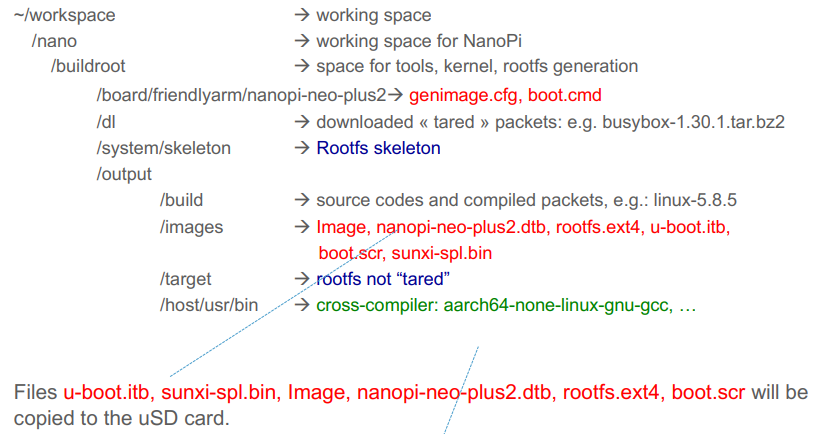
\includegraphics[width=\columnwidth]{img_1.png}
\end{figure}
Ce qui est manquant de le dossier output sera recompilé lorsque la commande \verb!make! est lancée (ou alors en faisant la commande \verb!make <package>-rebuild!.\\
Le dossier \verb!rootfs_overlay! permet d'ajouter des fichiers au \verb!rootfs!
(\verb!/workspace/nano/buildrootboard/friendlyarm/nanopi-neo-plus2/rootfs_overlay!)
\subsection{Compilation}
Dans le répertoire \verb!buildroot!, effectuer \verb!make menuconfig! puis \verb!make!. \verb!make clean! pour effacer tous les fichiers compilés.




\end{document}